% Options for packages loaded elsewhere
\PassOptionsToPackage{unicode}{hyperref}
\PassOptionsToPackage{hyphens}{url}
%
\documentclass[
]{article}
\usepackage{amsmath,amssymb}
\usepackage{iftex}
\ifPDFTeX
  \usepackage[T1]{fontenc}
  \usepackage[utf8]{inputenc}
  \usepackage{textcomp} % provide euro and other symbols
\else % if luatex or xetex
  \usepackage{unicode-math} % this also loads fontspec
  \defaultfontfeatures{Scale=MatchLowercase}
  \defaultfontfeatures[\rmfamily]{Ligatures=TeX,Scale=1}
\fi
\usepackage{lmodern}
\ifPDFTeX\else
  % xetex/luatex font selection
\fi
% Use upquote if available, for straight quotes in verbatim environments
\IfFileExists{upquote.sty}{\usepackage{upquote}}{}
\IfFileExists{microtype.sty}{% use microtype if available
  \usepackage[]{microtype}
  \UseMicrotypeSet[protrusion]{basicmath} % disable protrusion for tt fonts
}{}
\makeatletter
\@ifundefined{KOMAClassName}{% if non-KOMA class
  \IfFileExists{parskip.sty}{%
    \usepackage{parskip}
  }{% else
    \setlength{\parindent}{0pt}
    \setlength{\parskip}{6pt plus 2pt minus 1pt}}
}{% if KOMA class
  \KOMAoptions{parskip=half}}
\makeatother
\usepackage{xcolor}
\usepackage[margin=1in]{geometry}
\usepackage{color}
\usepackage{fancyvrb}
\newcommand{\VerbBar}{|}
\newcommand{\VERB}{\Verb[commandchars=\\\{\}]}
\DefineVerbatimEnvironment{Highlighting}{Verbatim}{commandchars=\\\{\}}
% Add ',fontsize=\small' for more characters per line
\usepackage{framed}
\definecolor{shadecolor}{RGB}{248,248,248}
\newenvironment{Shaded}{\begin{snugshade}}{\end{snugshade}}
\newcommand{\AlertTok}[1]{\textcolor[rgb]{0.94,0.16,0.16}{#1}}
\newcommand{\AnnotationTok}[1]{\textcolor[rgb]{0.56,0.35,0.01}{\textbf{\textit{#1}}}}
\newcommand{\AttributeTok}[1]{\textcolor[rgb]{0.13,0.29,0.53}{#1}}
\newcommand{\BaseNTok}[1]{\textcolor[rgb]{0.00,0.00,0.81}{#1}}
\newcommand{\BuiltInTok}[1]{#1}
\newcommand{\CharTok}[1]{\textcolor[rgb]{0.31,0.60,0.02}{#1}}
\newcommand{\CommentTok}[1]{\textcolor[rgb]{0.56,0.35,0.01}{\textit{#1}}}
\newcommand{\CommentVarTok}[1]{\textcolor[rgb]{0.56,0.35,0.01}{\textbf{\textit{#1}}}}
\newcommand{\ConstantTok}[1]{\textcolor[rgb]{0.56,0.35,0.01}{#1}}
\newcommand{\ControlFlowTok}[1]{\textcolor[rgb]{0.13,0.29,0.53}{\textbf{#1}}}
\newcommand{\DataTypeTok}[1]{\textcolor[rgb]{0.13,0.29,0.53}{#1}}
\newcommand{\DecValTok}[1]{\textcolor[rgb]{0.00,0.00,0.81}{#1}}
\newcommand{\DocumentationTok}[1]{\textcolor[rgb]{0.56,0.35,0.01}{\textbf{\textit{#1}}}}
\newcommand{\ErrorTok}[1]{\textcolor[rgb]{0.64,0.00,0.00}{\textbf{#1}}}
\newcommand{\ExtensionTok}[1]{#1}
\newcommand{\FloatTok}[1]{\textcolor[rgb]{0.00,0.00,0.81}{#1}}
\newcommand{\FunctionTok}[1]{\textcolor[rgb]{0.13,0.29,0.53}{\textbf{#1}}}
\newcommand{\ImportTok}[1]{#1}
\newcommand{\InformationTok}[1]{\textcolor[rgb]{0.56,0.35,0.01}{\textbf{\textit{#1}}}}
\newcommand{\KeywordTok}[1]{\textcolor[rgb]{0.13,0.29,0.53}{\textbf{#1}}}
\newcommand{\NormalTok}[1]{#1}
\newcommand{\OperatorTok}[1]{\textcolor[rgb]{0.81,0.36,0.00}{\textbf{#1}}}
\newcommand{\OtherTok}[1]{\textcolor[rgb]{0.56,0.35,0.01}{#1}}
\newcommand{\PreprocessorTok}[1]{\textcolor[rgb]{0.56,0.35,0.01}{\textit{#1}}}
\newcommand{\RegionMarkerTok}[1]{#1}
\newcommand{\SpecialCharTok}[1]{\textcolor[rgb]{0.81,0.36,0.00}{\textbf{#1}}}
\newcommand{\SpecialStringTok}[1]{\textcolor[rgb]{0.31,0.60,0.02}{#1}}
\newcommand{\StringTok}[1]{\textcolor[rgb]{0.31,0.60,0.02}{#1}}
\newcommand{\VariableTok}[1]{\textcolor[rgb]{0.00,0.00,0.00}{#1}}
\newcommand{\VerbatimStringTok}[1]{\textcolor[rgb]{0.31,0.60,0.02}{#1}}
\newcommand{\WarningTok}[1]{\textcolor[rgb]{0.56,0.35,0.01}{\textbf{\textit{#1}}}}
\usepackage{graphicx}
\makeatletter
\def\maxwidth{\ifdim\Gin@nat@width>\linewidth\linewidth\else\Gin@nat@width\fi}
\def\maxheight{\ifdim\Gin@nat@height>\textheight\textheight\else\Gin@nat@height\fi}
\makeatother
% Scale images if necessary, so that they will not overflow the page
% margins by default, and it is still possible to overwrite the defaults
% using explicit options in \includegraphics[width, height, ...]{}
\setkeys{Gin}{width=\maxwidth,height=\maxheight,keepaspectratio}
% Set default figure placement to htbp
\makeatletter
\def\fps@figure{htbp}
\makeatother
\setlength{\emergencystretch}{3em} % prevent overfull lines
\providecommand{\tightlist}{%
  \setlength{\itemsep}{0pt}\setlength{\parskip}{0pt}}
\setcounter{secnumdepth}{-\maxdimen} % remove section numbering
\ifLuaTeX
  \usepackage{selnolig}  % disable illegal ligatures
\fi
\usepackage{bookmark}
\IfFileExists{xurl.sty}{\usepackage{xurl}}{} % add URL line breaks if available
\urlstyle{same}
\hypersetup{
  pdftitle={Assignment1},
  pdfauthor={Yinghao Luo, Zheyuan Zhang, Yujie Cao},
  hidelinks,
  pdfcreator={LaTeX via pandoc}}

\title{Assignment1}
\author{Yinghao Luo, Zheyuan Zhang, Yujie Cao}
\date{2025-02-13}

\begin{document}
\maketitle

\subsection{Exercise 1}\label{exercise-1}

\textbf{(a)} For question 1a, we created several figures to check the
characteristics of the dataset, which include histogram, Q-Q plot.
According to the Q-Q plots, we can conclude that the data Before and
After both follow a normal distribution, since the plots is
approximately on a straight line.From the histogram,we can also make the
same conclusion.

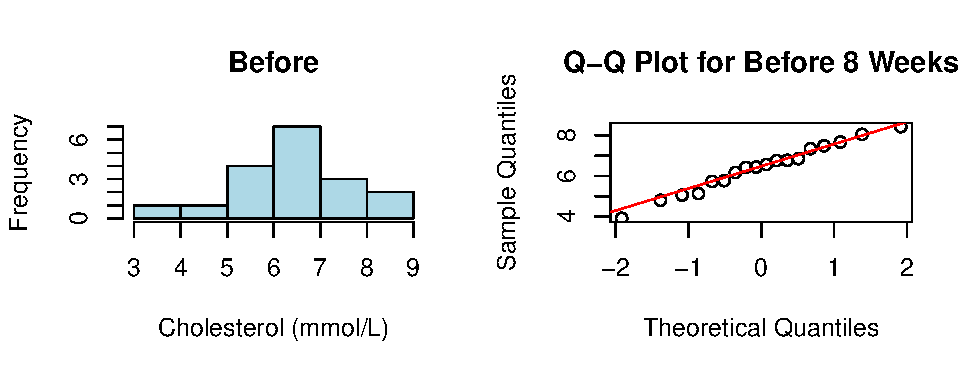
\includegraphics{assignment1-copy_files/figure-latex/unnamed-chunk-1-1.pdf}
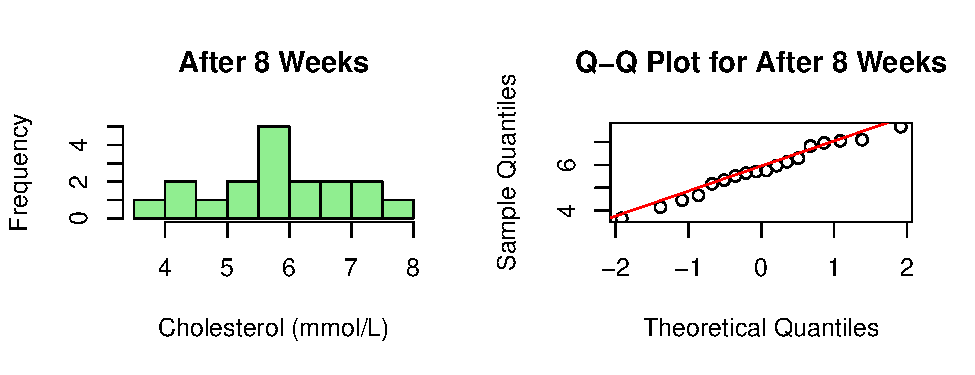
\includegraphics{assignment1-copy_files/figure-latex/unnamed-chunk-1-2.pdf}

Besides,we also check the scale,symmetry and outliers of the dataset
through boxplot.

\begin{Shaded}
\begin{Highlighting}[]
\FunctionTok{par}\NormalTok{(}\AttributeTok{mfrow =} \FunctionTok{c}\NormalTok{(}\DecValTok{1}\NormalTok{,}\DecValTok{2}\NormalTok{)) }
\FunctionTok{boxplot}\NormalTok{(data}\SpecialCharTok{$}\NormalTok{Before)}
\FunctionTok{boxplot}\NormalTok{(data}\SpecialCharTok{$}\NormalTok{After8weeks)}
\end{Highlighting}
\end{Shaded}

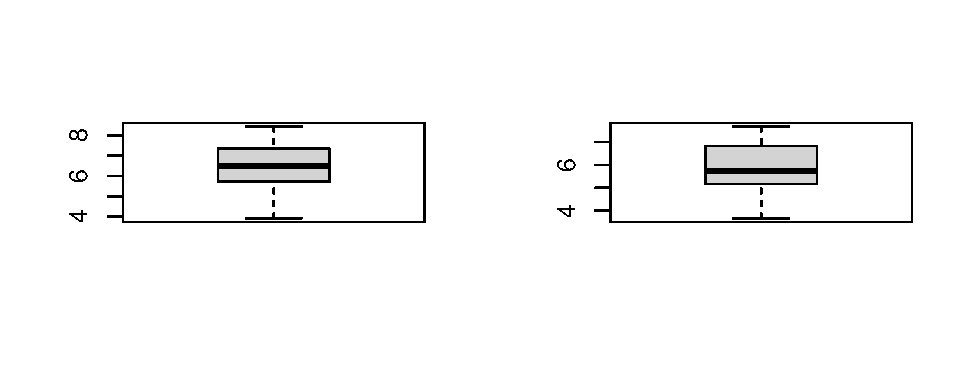
\includegraphics{assignment1-copy_files/figure-latex/unnamed-chunk-2-1.pdf}

\begin{Shaded}
\begin{Highlighting}[]
\FunctionTok{par}\NormalTok{(}\AttributeTok{mfrow =} \FunctionTok{c}\NormalTok{(}\DecValTok{1}\NormalTok{,}\DecValTok{1}\NormalTok{))}
\end{Highlighting}
\end{Shaded}

Then we also plot the scatter figures,we can see that there is
approximately linear relation between these two values.

\begin{Shaded}
\begin{Highlighting}[]
\CommentTok{\#length(data$Before)}
\CommentTok{\#length(data$After8weeks)}
\FunctionTok{plot}\NormalTok{(data}\SpecialCharTok{$}\NormalTok{Before, data}\SpecialCharTok{$}\NormalTok{After8weeks,}
     \AttributeTok{main =} \StringTok{"Scatter Plot of Before vs. After 8 Weeks"}\NormalTok{,}
     \AttributeTok{xlab =} \StringTok{"Before"}\NormalTok{, }\AttributeTok{ylab =} \StringTok{"After 8 Weeks"}\NormalTok{,}
     \AttributeTok{col =} \StringTok{"black"}\NormalTok{, }\AttributeTok{pch =} \DecValTok{16}\NormalTok{)}
\end{Highlighting}
\end{Shaded}

\includegraphics{assignment1-copy_files/figure-latex/unnamed-chunk-3-1.pdf}

The correlation of these two columns(Before and After) can also be
calculated by Pearson . Therefore, the value of correlation is 0.991,
which can infer that they are correlated with each other.

\begin{Shaded}
\begin{Highlighting}[]
\FunctionTok{cor.test}\NormalTok{(data}\SpecialCharTok{$}\NormalTok{Before, data}\SpecialCharTok{$}\NormalTok{After8weeks, }\AttributeTok{method=}\StringTok{"pearson"}\NormalTok{)}
\end{Highlighting}
\end{Shaded}

\begin{verbatim}
## 
##  Pearson's product-moment correlation
## 
## data:  data$Before and data$After8weeks
## t = 29, df = 16, p-value = 2e-15
## alternative hypothesis: true correlation is not equal to 0
## 95 percent confidence interval:
##  0.975 0.997
## sample estimates:
##   cor 
## 0.991
\end{verbatim}

To answer the question about if the data are paired or not, the answer
is yes. It is an experiment with two numerical outcomes per experimental
unit. To be specific, the data are measured at two different time
points, but within the same group of indiciduals. Therefore,
\textbf{Mann-Whitney test is not applicable}, because it is utilized to
compare two independent groups. However, the permutation test is
applicable since we do not assume normality in a permutation test. As
the sample size is 18,relatively small,we prefer non-Parametric tests.

First, we can conduct paired t-test as follows:

\begin{Shaded}
\begin{Highlighting}[]
\FunctionTok{t.test}\NormalTok{(data}\SpecialCharTok{$}\NormalTok{Before,data}\SpecialCharTok{$}\NormalTok{After8weeks, }\AttributeTok{paired=}\ConstantTok{TRUE}\NormalTok{)}
\end{Highlighting}
\end{Shaded}

\begin{verbatim}
## 
##  Paired t-test
## 
## data:  data$Before and data$After8weeks
## t = 15, df = 17, p-value = 3e-11
## alternative hypothesis: true mean difference is not equal to 0
## 95 percent confidence interval:
##  0.540 0.718
## sample estimates:
## mean difference 
##           0.629
\end{verbatim}

The p-value is 3e-11, so we can know taht \(H_0\) can be rejected.
\(H_0\) means no significant difference between Before and After8weeks.
In this case, there is significant difference between Before and
After8weeks.

Then, we can use permutation test as follows:

\begin{Shaded}
\begin{Highlighting}[]
\NormalTok{mean\_difference }\OtherTok{=} \ControlFlowTok{function}\NormalTok{(x,y) \{}\FunctionTok{mean}\NormalTok{(x}\SpecialCharTok{{-}}\NormalTok{y)\}}

\NormalTok{original\_diff }\OtherTok{\textless{}{-}} \FunctionTok{mean}\NormalTok{(data}\SpecialCharTok{$}\NormalTok{Before }\SpecialCharTok{{-}}\NormalTok{ data}\SpecialCharTok{$}\NormalTok{After8weeks)}

\NormalTok{B}\OtherTok{=}\DecValTok{1000}\NormalTok{; tstar}\OtherTok{=}\FunctionTok{numeric}\NormalTok{(B)}

\ControlFlowTok{for}\NormalTok{ (i }\ControlFlowTok{in} \DecValTok{1}\SpecialCharTok{:}\NormalTok{B) \{}
\NormalTok{  md\_star}\OtherTok{=}\FunctionTok{t}\NormalTok{(}\FunctionTok{apply}\NormalTok{(}\FunctionTok{cbind}\NormalTok{(data}\SpecialCharTok{$}\NormalTok{Before,data}\SpecialCharTok{$}\NormalTok{After8weeks),}\DecValTok{1}\NormalTok{,sample))}
\NormalTok{  tstar[i]}\OtherTok{=}\FunctionTok{mean\_difference}\NormalTok{(data}\SpecialCharTok{$}\NormalTok{Before,data}\SpecialCharTok{$}\NormalTok{After8weeks) }
\NormalTok{\}}

\NormalTok{myt }\OtherTok{=} \FunctionTok{mean\_difference}\NormalTok{(data}\SpecialCharTok{$}\NormalTok{Before,data}\SpecialCharTok{$}\NormalTok{After8weeks);myt}
\end{Highlighting}
\end{Shaded}

\begin{verbatim}
## [1] 0.629
\end{verbatim}

\begin{Shaded}
\begin{Highlighting}[]
\NormalTok{pl}\OtherTok{=}\FunctionTok{sum}\NormalTok{(tstar}\SpecialCharTok{\textless{}}\NormalTok{myt)}\SpecialCharTok{/}\NormalTok{B}
\NormalTok{pr}\OtherTok{=}\FunctionTok{sum}\NormalTok{(tstar}\SpecialCharTok{\textgreater{}}\NormalTok{myt)}\SpecialCharTok{/}\NormalTok{B}
\NormalTok{p}\OtherTok{=}\DecValTok{2}\SpecialCharTok{*}\FunctionTok{min}\NormalTok{(pl,pr); p}
\end{Highlighting}
\end{Shaded}

\begin{verbatim}
## [1] 0
\end{verbatim}

In the permutation test, we can reject \(H_0\) and the result also
demonstrates that the diet with low fat margarine has a significant
effect.

\textbf{c}

First, we construct the a 97\%-CI for \(\mu\) based on normality. As
\(X_1, \ldots, X_{18} \sim N(\mu,\sigma^2)\) , we can calculate the
t-confidence interval of level \(1-\alpha\) for \(\mu\) . Note,
\(\alpha\) is 3\% now.

\begin{Shaded}
\begin{Highlighting}[]
\NormalTok{x }\OtherTok{=}\NormalTok{ data}\SpecialCharTok{$}\NormalTok{After8weeks}
\NormalTok{n }\OtherTok{=} \FunctionTok{length}\NormalTok{(x)}
\NormalTok{x\_mean }\OtherTok{=} \FunctionTok{mean}\NormalTok{(x)}
\NormalTok{x\_sd }\OtherTok{=} \FunctionTok{sd}\NormalTok{(x) }
\NormalTok{alpha }\OtherTok{=} \FloatTok{0.03}

\NormalTok{t }\OtherTok{=} \FunctionTok{qt}\NormalTok{(}\DecValTok{1}\SpecialCharTok{{-}}\NormalTok{alpha}\SpecialCharTok{/}\DecValTok{2}\NormalTok{, }\AttributeTok{df =}\NormalTok{ n}\DecValTok{{-}1}\NormalTok{)}

\NormalTok{CI\_normal }\OtherTok{=} \FunctionTok{c}\NormalTok{(}
\NormalTok{  x\_mean }\SpecialCharTok{{-}}\NormalTok{ t }\SpecialCharTok{*}\NormalTok{ (x\_sd }\SpecialCharTok{/} \FunctionTok{sqrt}\NormalTok{(n)),}
\NormalTok{  x\_mean }\SpecialCharTok{+}\NormalTok{ t }\SpecialCharTok{*}\NormalTok{ (x\_sd }\SpecialCharTok{/} \FunctionTok{sqrt}\NormalTok{(n))}
\NormalTok{)}
\FunctionTok{cat}\NormalTok{(}\StringTok{"Normality 97\% confidence interval: ["}\NormalTok{, }\FunctionTok{round}\NormalTok{(CI\_normal[}\DecValTok{1}\NormalTok{], }\DecValTok{3}\NormalTok{), }
    \StringTok{","}\NormalTok{, }\FunctionTok{round}\NormalTok{(CI\_normal[}\DecValTok{2}\NormalTok{], }\DecValTok{3}\NormalTok{), }\StringTok{"]}\SpecialCharTok{\textbackslash{}n}\StringTok{"}\NormalTok{)}
\end{Highlighting}
\end{Shaded}

\begin{verbatim}
## Normality 97% confidence interval: [ 5.16 , 6.39 ]
\end{verbatim}

Then, we implement bootstrap CI as follows:

\begin{Shaded}
\begin{Highlighting}[]
\NormalTok{B }\OtherTok{=} \DecValTok{1000}
\NormalTok{x\_mean }\OtherTok{=} \FunctionTok{mean}\NormalTok{(data}\SpecialCharTok{$}\NormalTok{After8weeks)}
\NormalTok{Tstar }\OtherTok{=} \FunctionTok{numeric}\NormalTok{(B)}
\ControlFlowTok{for}\NormalTok{(i }\ControlFlowTok{in} \DecValTok{1}\SpecialCharTok{:}\NormalTok{B)\{}
\NormalTok{  Xstar}\OtherTok{=}\FunctionTok{sample}\NormalTok{(data}\SpecialCharTok{$}\NormalTok{After8weeks,}\AttributeTok{replace=}\ConstantTok{TRUE}\NormalTok{)}
\NormalTok{  Tstar[i]}\OtherTok{=}\FunctionTok{mean}\NormalTok{(Xstar)}
\NormalTok{\}}
\NormalTok{Tstar15 }\OtherTok{=} \FunctionTok{quantile}\NormalTok{(Tstar, }\FloatTok{0.015}\NormalTok{)}
\NormalTok{Tstar985 }\OtherTok{=} \FunctionTok{quantile}\NormalTok{(Tstar, }\FloatTok{0.985}\NormalTok{)}

\NormalTok{CI\_bootstrap }\OtherTok{=} \FunctionTok{c}\NormalTok{(}\DecValTok{2}\SpecialCharTok{*}\NormalTok{x\_mean}\SpecialCharTok{{-}}\NormalTok{Tstar985,}\DecValTok{2}\SpecialCharTok{*}\NormalTok{x\_mean}\SpecialCharTok{{-}}\NormalTok{Tstar15)}
\FunctionTok{cat}\NormalTok{(}\StringTok{"Bootstrap 97\% confidence interval: ["}\NormalTok{, }\FunctionTok{round}\NormalTok{(CI\_bootstrap[}\DecValTok{1}\NormalTok{], }\DecValTok{3}\NormalTok{), }
    \StringTok{","}\NormalTok{, }\FunctionTok{round}\NormalTok{(CI\_bootstrap[}\DecValTok{2}\NormalTok{], }\DecValTok{3}\NormalTok{), }\StringTok{"]}\SpecialCharTok{\textbackslash{}n}\StringTok{"}\NormalTok{)}
\end{Highlighting}
\end{Shaded}

\begin{verbatim}
## Bootstrap 97% confidence interval: [ 5.23 , 6.3 ]
\end{verbatim}

The difference between the two confidence intervals is slight. In my
view, this might be because after8weeks conforms to a normal
distribution.

\textbf{d}

We can use bootstrap method first as follows: The result may be slightly
different for each bootstrap test. We choose the maximum of the sample
as the test statistic and set B as 1000.

\begin{Shaded}
\begin{Highlighting}[]
\NormalTok{n}\OtherTok{=}\FunctionTok{length}\NormalTok{(data}\SpecialCharTok{$}\NormalTok{After8weeks) }\CommentTok{\# length}
\NormalTok{t}\OtherTok{=}\FunctionTok{max}\NormalTok{(data}\SpecialCharTok{$}\NormalTok{After8weeks) }\CommentTok{\# the max of samples}
\NormalTok{B}\OtherTok{=}\DecValTok{1000}\NormalTok{;}
\NormalTok{tstar}\OtherTok{=}\FunctionTok{numeric}\NormalTok{(B)}
\NormalTok{theta\_values }\OtherTok{=} \FunctionTok{seq}\NormalTok{(}\DecValTok{3}\NormalTok{, }\DecValTok{12}\NormalTok{, }\AttributeTok{by =} \FloatTok{0.1}\NormalTok{)}

\NormalTok{p\_values }\OtherTok{=} \FunctionTok{sapply}\NormalTok{(theta\_values, }\ControlFlowTok{function}\NormalTok{(theta) \{}
\NormalTok{  tstar }\OtherTok{=} \FunctionTok{numeric}\NormalTok{(B)}
  \ControlFlowTok{for}\NormalTok{ (i }\ControlFlowTok{in} \DecValTok{1}\SpecialCharTok{:}\NormalTok{B)\{}
\NormalTok{    xstar }\OtherTok{=} \FunctionTok{runif}\NormalTok{(n, }\AttributeTok{min =} \DecValTok{3}\NormalTok{, }\AttributeTok{max =}\NormalTok{ theta)}
\NormalTok{    tstar[i] }\OtherTok{=} \FunctionTok{max}\NormalTok{(xstar)}
\NormalTok{  \}}
\NormalTok{  pl }\OtherTok{=} \FunctionTok{sum}\NormalTok{(tstar }\SpecialCharTok{\textless{}}\NormalTok{ t) }\SpecialCharTok{/}\NormalTok{ B}
\NormalTok{  pr }\OtherTok{=} \FunctionTok{sum}\NormalTok{(tstar }\SpecialCharTok{\textgreater{}}\NormalTok{ t) }\SpecialCharTok{/}\NormalTok{ B}
\NormalTok{  p }\OtherTok{=} \DecValTok{2} \SpecialCharTok{*} \FunctionTok{min}\NormalTok{(pl, pr)}
  \FunctionTok{return}\NormalTok{(p)}
\NormalTok{\})}

\CommentTok{\# This is to find the range of theta for p \textgreater{} 0.05 }
\NormalTok{theta\_valid }\OtherTok{=}\NormalTok{ theta\_values[p\_values }\SpecialCharTok{\textgreater{}} \FloatTok{0.05}\NormalTok{]}

\FunctionTok{cat}\NormalTok{(}\StringTok{"The range of theta for H0 cannot be rejected: ["}\NormalTok{, }\FunctionTok{min}\NormalTok{(theta\_valid), }\FunctionTok{max}\NormalTok{(theta\_valid),  }\StringTok{"]}\SpecialCharTok{\textbackslash{}n}\StringTok{"}\NormalTok{)}
\end{Highlighting}
\end{Shaded}

\begin{verbatim}
## The range of theta for H0 cannot be rejected: [ 7.7 8.7 ]
\end{verbatim}

In terms of the question: Can the Kolmogorov-Smirnov test be also
applied for this question? My answer is no. The value of \(\theta\) is
not a known fixed value , so the empirical distribution function is not
completely known. In this case, it violates one of the assumptions of KS
test.

\textbf{e}

We can test whether the proportion of samples with cholesterol levels of
less than 6 are significantly less than 50\% after 8 weeks. We can set
the orginal hypothesis \(H_0\) : the median is 6, while \(H_1\) is
median is smaller than 6. The binomial test can be applied as follows:

\begin{Shaded}
\begin{Highlighting}[]
\NormalTok{n }\OtherTok{=} \FunctionTok{length}\NormalTok{(data}\SpecialCharTok{$}\NormalTok{After8weeks)}
\NormalTok{below\_6 }\OtherTok{=} \FunctionTok{sum}\NormalTok{(data}\SpecialCharTok{$}\NormalTok{After8weeks }\SpecialCharTok{\textless{}} \DecValTok{6}\NormalTok{);}

\FunctionTok{binom.test}\NormalTok{(below\_6,n,}\AttributeTok{p=}\FloatTok{0.5}\NormalTok{,}\AttributeTok{alt=}\StringTok{"l"}\NormalTok{)}
\end{Highlighting}
\end{Shaded}

\begin{verbatim}
## 
##  Exact binomial test
## 
## data:  below_6 and n
## number of successes = 11, number of trials = 18, p-value = 0.9
## alternative hypothesis: true probability of success is less than 0.5
## 95 percent confidence interval:
##  0.000 0.801
## sample estimates:
## probability of success 
##                  0.611
\end{verbatim}

Besides, we can also implement Wilcoxon signed rank test.

\begin{Shaded}
\begin{Highlighting}[]
 \FunctionTok{wilcox.test}\NormalTok{(data}\SpecialCharTok{$}\NormalTok{After8weeks,}\AttributeTok{mu=}\DecValTok{6}\NormalTok{)}
\end{Highlighting}
\end{Shaded}

\begin{verbatim}
## Warning in wilcox.test.default(data$After8weeks, mu = 6): cannot compute exact
## p-value with ties
\end{verbatim}

\begin{verbatim}
## 
##  Wilcoxon signed rank test with continuity correction
## 
## data:  data$After8weeks
## V = 68, p-value = 0.4
## alternative hypothesis: true location is not equal to 6
\end{verbatim}

We can conclude that \(H_0\) cannot be rejected, since the p-value is
higher than 0.05.

Let's forward to next question: design and perform a test to check
whether the fraction of the cholesterol levels after 8 weeks of low fat
diet less than 4.5 is at most 25\%.

We can set the original hypothesis \(H_0\) as the percentage of
cholesterol levels below 4.5 is less than 25\%, while \(H_1\) means the
percentage of cholesterol levels below 4.5 is more than or equal to
25\%.

\begin{Shaded}
\begin{Highlighting}[]
\NormalTok{below\_4}\FloatTok{.5} \OtherTok{=} \FunctionTok{sum}\NormalTok{(data}\SpecialCharTok{$}\NormalTok{After8weeks }\SpecialCharTok{\textless{}=} \FloatTok{4.5}\NormalTok{)}
\NormalTok{n }\OtherTok{=} \FunctionTok{length}\NormalTok{(data}\SpecialCharTok{$}\NormalTok{After8weeks)}

\CommentTok{\# check if percentage of cholesterol levels below 4.5 is greater then 25\%}
\FunctionTok{binom.test}\NormalTok{(below\_4}\FloatTok{.5}\NormalTok{,n,}\AttributeTok{p=}\FloatTok{0.25}\NormalTok{,}\AttributeTok{alt=}\StringTok{"greater"}\NormalTok{)}
\end{Highlighting}
\end{Shaded}

\begin{verbatim}
## 
##  Exact binomial test
## 
## data:  below_4.5 and n
## number of successes = 3, number of trials = 18, p-value = 0.9
## alternative hypothesis: true probability of success is greater than 0.25
## 95 percent confidence interval:
##  0.047 1.000
## sample estimates:
## probability of success 
##                  0.167
\end{verbatim}

Therefore, we cannot reject the original hypothesis \(H_0\) since the
p-value is larger than 0.05. We can conclude that the percentage of
cholesterol levels below 4.5 is at most 25\%.

\subsection{Exercise 2}\label{exercise-2}

\textbf{(a)} Before we perform relevant ANOVA models,we need to check
whether the data meets the necessary assumptions We need to check
normality for numeric columns.

\begin{Shaded}
\begin{Highlighting}[]
\NormalTok{df }\OtherTok{\textless{}{-}} \FunctionTok{read.table}\NormalTok{(}\StringTok{"crops.txt"}\NormalTok{, }\AttributeTok{header =} \ConstantTok{TRUE}\NormalTok{)}
\NormalTok{df}\SpecialCharTok{$}\NormalTok{County }\OtherTok{\textless{}{-}} \FunctionTok{as.factor}\NormalTok{(df}\SpecialCharTok{$}\NormalTok{County)}
\NormalTok{df}\SpecialCharTok{$}\NormalTok{Related }\OtherTok{\textless{}{-}} \FunctionTok{as.factor}\NormalTok{(df}\SpecialCharTok{$}\NormalTok{Related)}

\FunctionTok{shapiro.test}\NormalTok{(df}\SpecialCharTok{$}\NormalTok{Crops)}
\end{Highlighting}
\end{Shaded}

\begin{verbatim}
## 
##  Shapiro-Wilk normality test
## 
## data:  df$Crops
## W = 1, p-value = 0.3
\end{verbatim}

\begin{Shaded}
\begin{Highlighting}[]
\FunctionTok{shapiro.test}\NormalTok{(df}\SpecialCharTok{$}\NormalTok{Size)}
\end{Highlighting}
\end{Shaded}

\begin{verbatim}
## 
##  Shapiro-Wilk normality test
## 
## data:  df$Size
## W = 0.9, p-value = 0.001
\end{verbatim}

Since Anova is not robust to outliers,we first need to check if there
are outliers.

\begin{Shaded}
\begin{Highlighting}[]
\FunctionTok{boxplot}\NormalTok{(df}\SpecialCharTok{$}\NormalTok{Crops)}
\end{Highlighting}
\end{Shaded}

\includegraphics{assignment1-copy_files/figure-latex/unnamed-chunk-14-1.pdf}

We check variance equality using leveneTest before applying anova
model.As we can see p\textgreater0.05,thus we can apply anova models.

\begin{Shaded}
\begin{Highlighting}[]
\FunctionTok{library}\NormalTok{(car)}
\end{Highlighting}
\end{Shaded}

\begin{verbatim}
## Loading required package: carData
\end{verbatim}

\begin{Shaded}
\begin{Highlighting}[]
\FunctionTok{leveneTest}\NormalTok{(Crops }\SpecialCharTok{\textasciitilde{}}\NormalTok{ County, }\AttributeTok{data =}\NormalTok{ df)}
\end{Highlighting}
\end{Shaded}

\begin{verbatim}
## Levene's Test for Homogeneity of Variance (center = median)
##       Df F value Pr(>F)
## group  2     0.4   0.67
##       27
\end{verbatim}

\begin{Shaded}
\begin{Highlighting}[]
\FunctionTok{leveneTest}\NormalTok{(Crops }\SpecialCharTok{\textasciitilde{}}\NormalTok{ Related, }\AttributeTok{data =}\NormalTok{ df)}
\end{Highlighting}
\end{Shaded}

\begin{verbatim}
## Levene's Test for Homogeneity of Variance (center = median)
##       Df F value Pr(>F)
## group  1    1.09    0.3
##       28
\end{verbatim}

\begin{Shaded}
\begin{Highlighting}[]
\FunctionTok{leveneTest}\NormalTok{(Crops }\SpecialCharTok{\textasciitilde{}}\NormalTok{ County}\SpecialCharTok{:}\NormalTok{Related, }\AttributeTok{data =}\NormalTok{ df)}
\end{Highlighting}
\end{Shaded}

\begin{verbatim}
## Levene's Test for Homogeneity of Variance (center = median)
##       Df F value Pr(>F)
## group  5     0.3   0.91
##       24
\end{verbatim}

\textbf{ANOVA model} There are two main factors:Country and Related,we
also include the interaction factor:County+Related.

\textbf{Tests the independent effects}

\begin{Shaded}
\begin{Highlighting}[]
\NormalTok{anova\_model1 }\OtherTok{\textless{}{-}} \FunctionTok{aov}\NormalTok{(Crops }\SpecialCharTok{\textasciitilde{}}\NormalTok{ County }\SpecialCharTok{+}\NormalTok{ Related, }\AttributeTok{data =}\NormalTok{ df) }
\FunctionTok{summary}\NormalTok{(anova\_model1)}
\end{Highlighting}
\end{Shaded}

\begin{verbatim}
##             Df   Sum Sq Mean Sq F value Pr(>F)
## County       2 8.84e+06 4420721    0.82   0.45
## Related      1 2.38e+06 2378957    0.44   0.51
## Residuals   26 1.40e+08 5396286
\end{verbatim}

\textbf{Interaction model}

\begin{Shaded}
\begin{Highlighting}[]
\NormalTok{anova\_model2 }\OtherTok{\textless{}{-}} \FunctionTok{aov}\NormalTok{(Crops }\SpecialCharTok{\textasciitilde{}}\NormalTok{ County}\SpecialCharTok{*}\NormalTok{Related, }\AttributeTok{data =}\NormalTok{ df) }
\FunctionTok{summary}\NormalTok{(anova\_model2)}
\end{Highlighting}
\end{Shaded}

\begin{verbatim}
##                Df   Sum Sq Mean Sq F value Pr(>F)
## County          2 8.84e+06 4420721    0.76   0.48
## Related         1 2.38e+06 2378957    0.41   0.53
## County:Related  2 1.50e+06  748786    0.13   0.88
## Residuals      24 1.39e+08 5783578
\end{verbatim}

Since all p-values are large (≫ 0.05), we do not reject the null
hypotheses, meaning there is no strong evidence that County or Related
significantly impact Crops. As there is no significance for the
interaction model,we choose the pure model to estimate the data.

\begin{Shaded}
\begin{Highlighting}[]
\NormalTok{new\_farm }\OtherTok{\textless{}{-}} \FunctionTok{data.frame}\NormalTok{(}
  \AttributeTok{County =} \FunctionTok{factor}\NormalTok{(}\DecValTok{3}\NormalTok{, }\AttributeTok{levels =} \FunctionTok{c}\NormalTok{(}\DecValTok{1}\NormalTok{, }\DecValTok{2}\NormalTok{, }\DecValTok{3}\NormalTok{)), }
  \AttributeTok{Related =} \FunctionTok{factor}\NormalTok{(}\StringTok{"no"}\NormalTok{, }\AttributeTok{levels =} \FunctionTok{c}\NormalTok{(}\StringTok{"no"}\NormalTok{, }\StringTok{"yes"}\NormalTok{))}
\NormalTok{)}

\NormalTok{predicted\_crops }\OtherTok{\textless{}{-}} \FunctionTok{predict}\NormalTok{(anova\_model1, }\AttributeTok{newdata =}\NormalTok{ new\_farm, }\AttributeTok{interval =} \StringTok{"confidence"}\NormalTok{)}
\FunctionTok{print}\NormalTok{(predicted\_crops)}
\end{Highlighting}
\end{Shaded}

\begin{verbatim}
##    fit  lwr  upr
## 1 7760 6017 9504
\end{verbatim}

Here we do the post-hoc check using TukeyHSD

\begin{Shaded}
\begin{Highlighting}[]
\FunctionTok{TukeyHSD}\NormalTok{(anova\_model2)}
\end{Highlighting}
\end{Shaded}

\begin{verbatim}
##   Tukey multiple comparisons of means
##     95% family-wise confidence level
## 
## Fit: aov(formula = Crops ~ County * Related, data = df)
## 
## $County
##     diff   lwr  upr p adj
## 2-1 -317 -3003 2369 0.953
## 3-1  960 -1726 3646 0.650
## 3-2 1277 -1409 3963 0.472
## 
## $Related
##        diff   lwr  upr p adj
## yes-no -563 -2376 1249 0.527
## 
## $`County:Related`
##              diff   lwr  upr p adj
## 2:no-1:no      93 -4610 4796 1.000
## 3:no-1:no     851 -3852 5554 0.993
## 1:yes-1:no   -362 -5065 4341 1.000
## 2:yes-1:no  -1090 -5792 3613 0.978
## 3:yes-1:no    706 -3997 5409 0.997
## 3:no-2:no     758 -3945 5461 0.996
## 1:yes-2:no   -455 -5158 4248 1.000
## 2:yes-2:no  -1183 -5885 3520 0.969
## 3:yes-2:no    613 -4090 5316 0.998
## 1:yes-3:no  -1213 -5916 3490 0.965
## 2:yes-3:no  -1941 -6644 2762 0.795
## 3:yes-3:no   -145 -4848 4558 1.000
## 2:yes-1:yes  -728 -5430 3975 0.997
## 3:yes-1:yes  1068 -3635 5771 0.980
## 3:yes-2:yes  1796 -2907 6499 0.842
\end{verbatim}

The Tukey test results confirm that the differences in means are not
statistically significant.

Examining residuals can help assess if the model assumptions hold. We
can see that it shows non-random pattern,which suggests that the model
is not well-fitted and may omit variables.

We can see that residuals are normally distributed.

\begin{Shaded}
\begin{Highlighting}[]
\NormalTok{residuals1 }\OtherTok{\textless{}{-}} \FunctionTok{resid}\NormalTok{(anova\_model1)}
\NormalTok{fitted\_values1 }\OtherTok{\textless{}{-}} \FunctionTok{fitted}\NormalTok{(anova\_model1) }
\FunctionTok{qqnorm}\NormalTok{(residuals1)}
\end{Highlighting}
\end{Shaded}

\includegraphics{assignment1-copy_files/figure-latex/unnamed-chunk-20-1.pdf}

\begin{Shaded}
\begin{Highlighting}[]
\CommentTok{\#length(fitted\_values1)}
\CommentTok{\#length(residuals)}
\CommentTok{\#class(fitted\_values1)}
\CommentTok{\#class(residuals)}
\FunctionTok{plot}\NormalTok{(fitted\_values1,residuals1 , }\AttributeTok{main =} \StringTok{"Residuals vs. Fitted"}\NormalTok{, }
     \AttributeTok{xlab =} \StringTok{"Fitted Values"}\NormalTok{, }\AttributeTok{ylab =} \StringTok{"Residuals"}\NormalTok{, }\AttributeTok{pch =} \DecValTok{19}\NormalTok{)}
\FunctionTok{abline}\NormalTok{(}\AttributeTok{h =} \DecValTok{0}\NormalTok{, }\AttributeTok{col =} \StringTok{"red"}\NormalTok{, }\AttributeTok{lty =} \DecValTok{2}\NormalTok{)}
\end{Highlighting}
\end{Shaded}

\includegraphics{assignment1-copy_files/figure-latex/unnamed-chunk-21-1.pdf}

\textbf{(b)} ANOVA models only assumes that crops only depend on
categorical factors,put size into perspective, we consider different
ANCOVA models:

\begin{Shaded}
\begin{Highlighting}[]
\FunctionTok{boxplot}\NormalTok{(df}\SpecialCharTok{$}\NormalTok{Size,}\AttributeTok{horizontal =} \ConstantTok{TRUE}\NormalTok{)}
\end{Highlighting}
\end{Shaded}

\includegraphics{assignment1-copy_files/figure-latex/unnamed-chunk-22-1.pdf}

\textbf{Tests the independent effects}

\begin{Shaded}
\begin{Highlighting}[]
\NormalTok{ancova\_main }\OtherTok{\textless{}{-}} \FunctionTok{aov}\NormalTok{(Crops }\SpecialCharTok{\textasciitilde{}}\NormalTok{ County }\SpecialCharTok{+}\NormalTok{ Related }\SpecialCharTok{+}\NormalTok{ Size, }\AttributeTok{data =}\NormalTok{ df)}
\FunctionTok{summary}\NormalTok{(ancova\_main)}
\end{Highlighting}
\end{Shaded}

\begin{verbatim}
##             Df   Sum Sq  Mean Sq F value  Pr(>F)    
## County       2 8.84e+06 4.42e+06    3.71   0.039 *  
## Related      1 2.38e+06 2.38e+06    2.00   0.170    
## Size         1 1.10e+08 1.10e+08   92.68 6.9e-10 ***
## Residuals   25 2.98e+07 1.19e+06                    
## ---
## Signif. codes:  0 '***' 0.001 '**' 0.01 '*' 0.05 '.' 0.1 ' ' 1
\end{verbatim}

\textbf{Size × County Interaction}

\begin{Shaded}
\begin{Highlighting}[]
\NormalTok{ancova\_county\_size }\OtherTok{\textless{}{-}} \FunctionTok{aov}\NormalTok{(Crops }\SpecialCharTok{\textasciitilde{}}\NormalTok{ County }\SpecialCharTok{*}\NormalTok{ Size }\SpecialCharTok{+}\NormalTok{ Related, }\AttributeTok{data =}\NormalTok{ df)}
\FunctionTok{summary}\NormalTok{(ancova\_county\_size)}
\end{Highlighting}
\end{Shaded}

\begin{verbatim}
##             Df   Sum Sq  Mean Sq F value Pr(>F)    
## County       2 8.84e+06 4.42e+06    5.01  0.016 *  
## Size         1 1.11e+08 1.11e+08  126.47  8e-11 ***
## Related      1 1.38e+06 1.38e+06    1.57  0.223    
## County:Size  2 9.53e+06 4.76e+06    5.40  0.012 *  
## Residuals   23 2.03e+07 8.82e+05                   
## ---
## Signif. codes:  0 '***' 0.001 '**' 0.01 '*' 0.05 '.' 0.1 ' ' 1
\end{verbatim}

\textbf{Size × Related Interaction}

\begin{Shaded}
\begin{Highlighting}[]
\NormalTok{ancova\_related\_size }\OtherTok{\textless{}{-}} \FunctionTok{aov}\NormalTok{(Crops }\SpecialCharTok{\textasciitilde{}}\NormalTok{ County }\SpecialCharTok{+}\NormalTok{ Related }\SpecialCharTok{*}\NormalTok{ Size, }\AttributeTok{data =}\NormalTok{ df)}
\FunctionTok{summary}\NormalTok{(ancova\_related\_size)}
\end{Highlighting}
\end{Shaded}

\begin{verbatim}
##              Df   Sum Sq  Mean Sq F value  Pr(>F)    
## County        2 8.84e+06 4.42e+06    3.73   0.039 *  
## Related       1 2.38e+06 2.38e+06    2.01   0.169    
## Size          1 1.10e+08 1.10e+08   93.21 9.7e-10 ***
## Related:Size  1 1.35e+06 1.35e+06    1.14   0.296    
## Residuals    24 2.85e+07 1.19e+06                    
## ---
## Signif. codes:  0 '***' 0.001 '**' 0.01 '*' 0.05 '.' 0.1 ' ' 1
\end{verbatim}

\begin{Shaded}
\begin{Highlighting}[]
\FunctionTok{AIC}\NormalTok{(ancova\_main, ancova\_county\_size, ancova\_related\_size)}
\end{Highlighting}
\end{Shaded}

\begin{verbatim}
##                     df AIC
## ancova_main          6 511
## ancova_county_size   8 504
## ancova_related_size  7 512
\end{verbatim}

We can see from p-values that Size × County interaction terms is
significant and this model have low AIC,thus we choose Size × County
Interaction model.

\textbf{(c)} We can review the ANCOVA Model Results.

Significant County (p \textless{} 0.05) → County influences on
Crops,meaning crop yields differ across counties..

Significant Size (p \textless{} 0.05) → Farm Size has a strong effect on
Crops,which makes sense---larger farms generally produce more.

Significant Related (p \textgreater{} 0.05) → Whether the landlord and
tenant are related does not significantly impact the crops.

Significant County × Size (p \textless{} 0.05) → This suggests that the
effect of farm size on crop yield depends on the county. The figure blow
confirms this conclusion,as the slopes are different.

\begin{Shaded}
\begin{Highlighting}[]
\FunctionTok{library}\NormalTok{(ggplot2)}
\FunctionTok{ggplot}\NormalTok{(df, }\FunctionTok{aes}\NormalTok{(}\AttributeTok{x =}\NormalTok{ Size, }\AttributeTok{y =}\NormalTok{ Crops, }\AttributeTok{color =}\NormalTok{ County)) }\SpecialCharTok{+}
  \FunctionTok{geom\_point}\NormalTok{() }\SpecialCharTok{+}
  \FunctionTok{geom\_smooth}\NormalTok{(}\AttributeTok{method =} \StringTok{"lm"}\NormalTok{, }\AttributeTok{se =} \ConstantTok{FALSE}\NormalTok{) }\SpecialCharTok{+}
  \FunctionTok{labs}\NormalTok{(}\AttributeTok{title =} \StringTok{"Effect of Size on Crops Across Counties"}\NormalTok{,}
       \AttributeTok{x =} \StringTok{"Farm Size"}\NormalTok{, }\AttributeTok{y =} \StringTok{"Crops Yield"}\NormalTok{)}
\end{Highlighting}
\end{Shaded}

\begin{verbatim}
## `geom_smooth()` using formula = 'y ~ x'
\end{verbatim}

\includegraphics{assignment1-copy_files/figure-latex/unnamed-chunk-27-1.pdf}

\textbf{(d)}

\begin{Shaded}
\begin{Highlighting}[]
\NormalTok{new\_farm }\OtherTok{\textless{}{-}} \FunctionTok{data.frame}\NormalTok{(}
  \AttributeTok{County =} \FunctionTok{factor}\NormalTok{(}\DecValTok{2}\NormalTok{, }\AttributeTok{levels =} \FunctionTok{c}\NormalTok{(}\DecValTok{1}\NormalTok{, }\DecValTok{2}\NormalTok{, }\DecValTok{3}\NormalTok{)), }
  \AttributeTok{Related =} \FunctionTok{factor}\NormalTok{(}\StringTok{"yes"}\NormalTok{, }\AttributeTok{levels =} \FunctionTok{c}\NormalTok{(}\StringTok{"no"}\NormalTok{, }\StringTok{"yes"}\NormalTok{)),}
  \AttributeTok{Size =} \DecValTok{165}  
\NormalTok{)}

\NormalTok{predicted\_crops }\OtherTok{\textless{}{-}} \FunctionTok{predict}\NormalTok{(ancova\_county\_size, }\AttributeTok{newdata =}\NormalTok{ new\_farm, }\AttributeTok{interval =} \StringTok{"confidence"}\NormalTok{)}
\FunctionTok{print}\NormalTok{(predicted\_crops)}
\end{Highlighting}
\end{Shaded}

\begin{verbatim}
##    fit  lwr  upr
## 1 6141 5428 6855
\end{verbatim}

We can see that residuals are approximately normally distributed.

\begin{Shaded}
\begin{Highlighting}[]
\NormalTok{residuals }\OtherTok{\textless{}{-}} \FunctionTok{resid}\NormalTok{(ancova\_county\_size)}
\NormalTok{fitted\_values }\OtherTok{\textless{}{-}} \FunctionTok{fitted}\NormalTok{(ancova\_county\_size) }
\FunctionTok{qqnorm}\NormalTok{(residuals)}
\FunctionTok{qqline}\NormalTok{(residuals, }\AttributeTok{col =} \StringTok{"red"}\NormalTok{)}
\end{Highlighting}
\end{Shaded}

\includegraphics{assignment1-copy_files/figure-latex/unnamed-chunk-29-1.pdf}

\begin{Shaded}
\begin{Highlighting}[]
\CommentTok{\#length(fitted\_values)}
\CommentTok{\#length(residuals)}
\FunctionTok{plot}\NormalTok{(fitted\_values, residuals, }
     \AttributeTok{main =} \StringTok{"Residuals vs Fitted Values"}\NormalTok{, }
     \AttributeTok{xlab =} \StringTok{"Fitted Values"}\NormalTok{, }
     \AttributeTok{ylab =} \StringTok{"Residuals"}\NormalTok{)}
\FunctionTok{abline}\NormalTok{(}\AttributeTok{h =} \DecValTok{0}\NormalTok{, }\AttributeTok{col =} \StringTok{"red"}\NormalTok{, }\AttributeTok{lty =} \DecValTok{2}\NormalTok{)}
\end{Highlighting}
\end{Shaded}

\includegraphics{assignment1-copy_files/figure-latex/unnamed-chunk-30-1.pdf}

We estimate the error variance.

\begin{Shaded}
\begin{Highlighting}[]
\NormalTok{error\_variance }\OtherTok{\textless{}{-}} \FunctionTok{sum}\NormalTok{(}\FunctionTok{residuals}\NormalTok{(ancova\_county\_size)}\SpecialCharTok{\^{}}\DecValTok{2}\NormalTok{) }\SpecialCharTok{/} \FunctionTok{df.residual}\NormalTok{(ancova\_county\_size)}
\FunctionTok{print}\NormalTok{(error\_variance)}
\end{Highlighting}
\end{Shaded}

\begin{verbatim}
## [1] 881623
\end{verbatim}

\end{document}
